\section{اطلاعات اولیه}
با توجه به مهم بودن بحث آلودگی هوا به خصوص در ایران و مشکلاتی که در سال‌های اخیر ایجاد کرده، تصمیم گرفتیم سامانه‌ای بسازیم که بتواند کیفیت محلی هوا را گزارش کند  و علاوه بر سادگی در هر جایی قابل استفاده باشد. در واقع ایده‌ی اصلی این پروژه این است که به جای استفاده از تعداد محدودی پایگاه اندازه‌گیری وضعیت هوا در سطح شهر، یک سامانه‌ی ساده و کاربردی در هر ساختمان یا آپارتمان باشد که علاوه بر بررسی وضعیت هوای بیرون، بتوانیم وجود گاز‌های سمی (مثلا در اثر نشت گاز) در داخل مکان بسته را نیز به سادگی تشخیص دهیم. در این صورت هر فردی می‌تواند از وضعیت هوای اطراف خودش مطلع شود و بر‌اساس آن اقدامات ضروری را انجام دهد. 

در این بخش با اطلاعات اولیه پروژه و کلیت عملکرد و هدف از ارائه این سیستم آشنا می‌شویم. 
\subsection{عنوان}
طراحی سامانه رصد وضعیت هوا
\subsection{حوزه کاربردی}
در طراحی ساختمان‌های ایمن و هوشمند و هم‌چنین در حوزه تحقیقات در زمینه کیفیت هوا
\subsection{هدف}
اندازه‌گیری شاخص‌های وضعیت هوا و گزارش آن‌ها بصورت آنلاین و ارائه اخطار‌های لازم در صورت وجود درصد بالای گاز‌های سمی



\section{شرح پروژه}

پس از این‌که در بخش اول با محصول نهایی و عملکرد کلی آن به صورت مختصر آشنا شدید، در این بخش می‌خواهیم نحوه عملکرد محصول نهایی را به همراه مراحلی که برای ساخت آن طی می‌شود، توضیح دهیم. توجه کنید که اولین مرحله برای ساخت دستگاه شناخت چگونگی عملکرد آن است. پس از شناخت صحیح عملکرد دستگاه، برمبنای عملکرد آن یک دیاگرام بلوکی برای آن طراحی می‌کنیم و در نهایت به کمک این دیاگرام، مراحل ساخت ماژول‌های مختلف و در نهایت ساخت دستگاه نهایی را بیان خواهیم کرد.

\subsection{چگونگی عملکرد دستگاه}

دستگاه ذکر شده 
\textbf{سه}
سنسور مهم خواهد داشت:

\begin{itemize}
	\item
	\textbf{سنسور کیفیت هوا:} 
	این سنسور که سنسور
	\lr{MQ-135}
	نام دارد، تمرکز گازهای احتراق‌پذیر در بخشی از هوا را تشخیص می‌دهد. رسانایی این سنسور در هوای پاک کم است در حالی که رسانایی آن با وجود گازهای قابل سوختن در هوا افزایش پیدا می‌کند. این سنسور به بخارات آمونیاک، بنزن و سولفید حساس است و مقادیر آن‌ها از ۱۰۰ الی ۱۰۰۰ 
	\lr{ppm}
	را تشخیص می‌دهد. لازم به ذکر است که از آنجا که این سنسور در \lr{Proteus} وجود ندارد ما برای شبیه‌سازی از سنسور جایگزین استفاده می‌کنیم. 
	
	\item
	\textbf{سنسور تشخیص مونوکسید کربن:}
	این سنسور که سنسور
	\lr{MQ-7}
	در آردوینو است، میزان مونوکسید کربن را در هوا تشخیص می‌دهد. ماده تشخیص دهنده به کار رفته در این سنسور، اکسید قلع است و هنگام تراکم گاز مونوکسید کربن در هوا، رسانایی این سنسور افزایش می‌یابد.
	
	\item
	\textbf{سنسور تشخیص دود و مشتقات گاز طبیعی:}
	این سنسور که سنسور
	\lr{MQ-2}
	است نیز تقریبا عملکردی مشابه سایر سنسور‌های قبلی دارد و با افزایش و تراکم دود و یا مشتقات گاز طبیعی از هوا، رسانایی آن بیشتر شده و وجود مقدار زیاد این گازها را تشخیص می‌دهد.
\end{itemize}

حال که عملکرد سنسور‌های دستگاه را توضیح دادیم، به توضیح عملکرد کلی دستگاه می‌پردازیم. این دستگاه از سه سنسور ذکر شده در بالا تشکیل شده است که همگی متصل به برد آردوینو هستند. حال سنسور‌ها اطلاعات گازهای مهم هوا را استخراج کرده و به برد آردوینو منتقل می‌کنند. سپس این اطلاعات کسب شده که حاوی میزان غلظت گازهای مختلف در هوا
بر حسب 
\lr{ppm}
است،
توسط برد آردوینو و کد نوشته شده در آن تحلیل می‌شود و در نهایت اطلاعات کسب شده از محیط پس از انجام محاسبات تعدادی عدد ملموس به ما خواهند داد. حال یک اپلیکیشن ساده موبایل خواهیم نوشت که این اطلاعات عددی ملموس را در یک قالب کاربرپسند به دیگران نشان دهد.
\subsection{بلوک دیاگرام ماژول‌ها}

ماژول‌های کلی در این دستگاه عبارتند از سه سنسور مربوطه که به برد آردوینو متصل می‌شوند و در نهایت نیز برد آردوینو به موبایل و اپلیکیشن مربوطه وصل خواهد شد و اطلاعات را درون اپلیکیشن نمایش خواهد داد. بلوک دیاگرام کلی ماژول‌ها را می‌توان به صورت زیر رسم نمود: 

\begin{figure}[h!]
	\centering		
	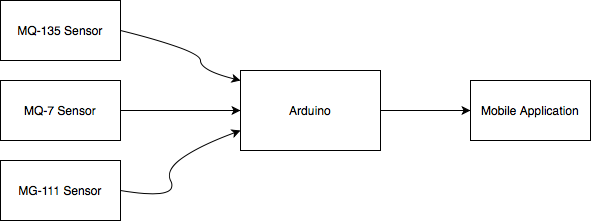
\includegraphics[width=0.8\linewidth]{1.png}
	\caption{دیاگرام بلوکی ماژول‌ها}
	\label{fig:boat1}
\end{figure}

همچنین با استفاده از نرم‌افزار 
fritzing
سیستم نهایی (بدون شبیه‌سازی) را پیاده‌سازی کردیم که نحوه‌ی اتصال ماژول‌ها و ورودی و خروجی‌های سنسور‌ها و پورت‌های برد آردوینو بهتر مشخص شود.  در بخش بعد در رابطه با پورت‌های گوناگون سنسور‌ها که در شکل زیر دیده می‌شود بیشتر توضیج می‌دهیم. 

\begin{figure}[h!]
	\centering		
	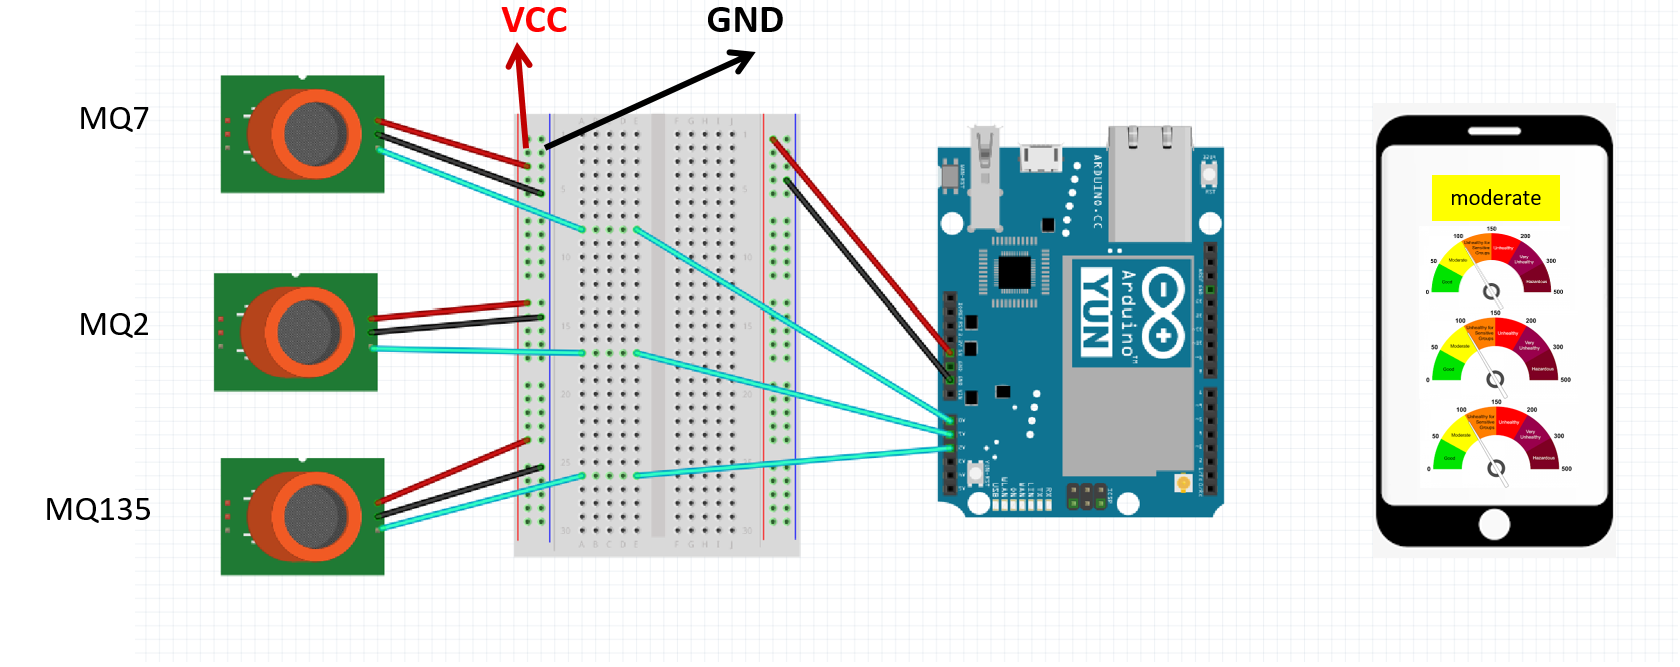
\includegraphics[width=\linewidth]{sys.png}
	\caption{نحوه‌ی اتصال اجزا در سیستم}
	\label{fig:boat1}
\end{figure}


\subsection{مراحل ساخت دستگاه}

مرحله اول ساخت دستگاه، اتصال صحیح سنسور‌ها به برد آردوینو است. هر یک از این سه سنسور، دارای سه پین مختلف است. پین 
\lr{VCC}
هر سه سنسور را باید به بین 
\lr{5V}
در آردوینو متصل کنیم و هم‌چنین پین 
\lr{GND}
در هر یک از سه سنسور باید به پین 
\lr{GND}
آردوینو متصل شود. حال این سنسور‌ها یک پین 
\lr{SIG}
نیز دارند که پین 
\lr{SIG}
سنسور کیفیت هوا را به پین 
\lr{A3}
آردوینو، پین 
\lr{SIG}
سنسور تشخیص کربن مونوکسید را به پین
\lr{A2}
در آردوینو و در نهایت پین تشخیص کربن دی‌اکسید را به پین 
\lr{A1}
در آردوینو متصل می‌کنیم. پس از اتصال سنسور‌ها، تمامی این سنسور‌ها میزان گاز در هوا را به صورت میزان ولتاژ عبوری و یا همان رسانایی نشان می‌دهند. در این جا باید از کتابخانه‌هایی برای تبدیل این میزان ولتاژ به غلظت گازها برحسب 
\lr{ppm}
استفاده کنیم. 
\paragraph{}
پس از این که غلظت گازها به دست آمد، باید براساس این غلظت‌ها شاخص آلودگی هوا را محاسبه کنیم. پس از انجام این محاسبات ریاضی توسط کد‌ها و کتابخانه‌های آردوینو، اعدادی مانند غلظت گاز مورد نظر یا شاخص آلودگی هوا که می‌خواهیم نشان داده شوند را در کد در نظر گرفته و سپس این کد را به یک اپلیکیشن موبایل متصل می‌کنیم. در اپلیکیشن این اعداد در یک محیط زیبا و کاربرپسند به شخص نشان داده خواهند شد. درنهایت بر اساس غلظت گاز‌های مختلف، وضعیت کلی هوا در یکی از دسته‌های زیر قرار می‌گیرد. این دسته‌بندی بر‌اساس استاندارد‌های سازمان بهداشت جهانی در نظر گرفته شده است. 
\begin{figure}[h!]
	\centering	
	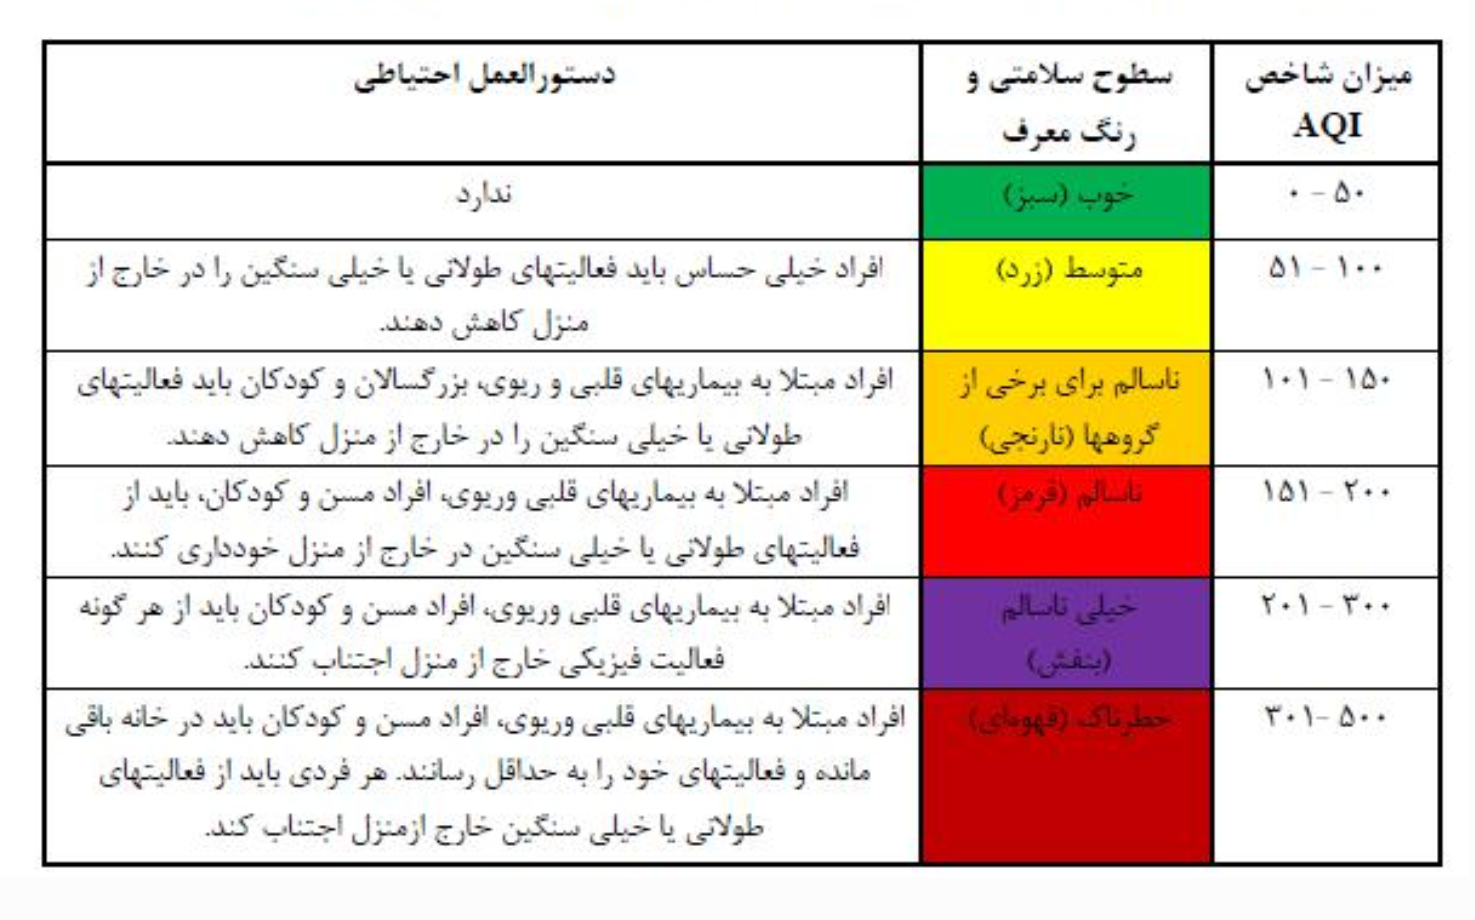
\includegraphics[width=0.8\linewidth]{farsiaqi.png}
	\caption{شاخص عددی آلودگی هوا برای گاز}
	\label{fig:boat1}
\end{figure} 

که البته ما در اینجا تنها تعدادی از این گاز‌ها را در نظر می‌گیریم. همانطور که دیده می‌شود در نهایت وضعیت آلودگی با یکی از شش رنگ سبز، زرد، نارنجی، قرمز، بنفش و زرشگی در اپلیکیشن مشخص می‌شود.  
\subsubsection{فاز‌بندی پروژه}
بنابراین به طور کلی فاز‌بندی پروژه به شرح زیر می‌شود:
\begin{enumerate}
	\item 
	\textbf{ طراحی کلی سیستم و ارائه پروپوزال:}
	در این فاز در رابطه با کاربرد‌های گوناگون سیستم‌های نهفته تحقیق کرده و با برد‌های مختلف آشنا شدیم و مقدمات برنامه‌نویسی آردینو و ساخت سیستم نهفته را نیز از کلاس درس فراگرفتیم. در نهایت طرح کلی از سیستم ارائه دادیم و پروپوزال را نوشتیم.	
	
	\item 
	\textbf{ یادگیری ابزار‌های لازم:}
	فاز دوم یادگیری برنامه‌نویسی اندروید در حدی که برای ساخت اپلیکیشن موبایل نیاز داریم و همچنین کار با iotBuilder نرم‌افزار شبیه‌ساز پروتئوس است که از آن برای ارتباط wireless با اپلیکیشن گوشی استفاده می‌شود. البته هدف اولیه این بود که از کتاب‌خانه‌ی
	thinger
	خود آردینو استفاده کنیم و برد را مستقیم به اپلیکیشن متصل کنیم اما با توجه به شرایط موجود و این که قرار است پروژه به صورت شبیه سازی ارائه شود تصمیم گرفتیم از 
	Visual Designer 
	پروتئوس استفاده کنیم.   
	\item 
	
	\textbf{نوشتن کد‌های لازم آردوینو و شبیه‌سازی در پروتئوس :}
	در فاز سوم کل کد‌های لازم در آردینو را نوشته و شبیه‌سازی‌ را انجام می‌دهیم. این کار شامل تحلیل عددی خروجی سنسور‌ها نیز می‌شود.  
	\item 
	
	\textbf{پیاده‌سازی سیستم و سیمولیشن نهایی :}
	این فاز به نوعی با فاز سوم در ارتباط است و هدف این بود اگر بتوانیم سنسور‌ها و برد لازم را تهیه کنیم، خود سیستم را پیاده‌سازی کنیم. در غیر این صورت این فاز تکمیل فاز سوم خواهد بود. 
	\item 
	\textbf{ طراحی اپلیکیش موبایل :}
	در نهایت در فاز آخر یک اپلیکیشن موبایل طراحی می‌کنیم که وضعیت گاز‌های مختلف و شاخص کیفت هوا (AQI) ،اقداماتی که کاربر در صورت نامناسب بودن وضعیت هوا باید پیش بگیرد را به اون گزارش کند. 	
\end{enumerate}
\pagebreak
\section{تقسیم وظایف}
به طور کلی تمام افراد در پنج فازی که در بخش قبل ذکر کردیم همکاری می‌کنند اما برای هر بخش مسئولانی اصلی در نظر گرفتیم که روند پروژه در آن فاز را مدیریت کنند. 

\begin{table}[ht]
	\begin{center}
		\begin{tabular}{|c|c|c|}
			\hline
			فاز & مسئولین اصلی & افراد مشارکت‌کننده\\
			\hline
			\hline
			1 & یاسمین طباطبایی - سروش باسلی‌زاده & هر سه عضو \\
			\hline
			2 & کوشا جافریان & هر سه عضو \\
			\hline
			3 & یاسمین طباطبایی  & هر سه عضو \\
			\hline
			3 & سروش باسلی‌زاده - کوشا جافریان  & هر سه عضو \\
			\hline
			3 & هر سه عضو  & هر سه عضو \\
			\hline
		\end{tabular}
	\end{center}	
\end{table}

\section{زمان‌بندی}
با توجه به مراحل ذکر شده در بخش 2.3، در این بخش زمان‌بندی انجام هر مرحله را به طور حدودی مشخص کرده ایم.  زمان کل پروژه مدت 4 ماه از 10 اسفند تا 10 تیر ماه در نظر گرفته شده است و فعالیت‌ها هفتگی دسته‌بندی شده‌اند. 

\begin{table}[ht]
	\begin{center}
		\begin{tabular}{|c|c|c|}
			\hline
			
			هفته & فاز & فعالیت\\
			\hline
			\hline
			10 اسفند - 16 اسفند & فاز 1 &  تحقیق در رابطه با سیستم‌های نهفته مختلف و انتخاب موضوع\\												
			\hline
			17 اسفند - 23 اسفند & فاز 1 &  آشنایی با بردهای آردوینو و چگونگی برنامه‌نویسی آن\\												
			\hline
			24 اسفند - 29 اسفند & فاز 1 &  نهایی کردن طرح کلی پیاده‌سازی سیستم\\												
			
			\hline
			تعطیلات سال جدید & - &  -\\															
			\hline
			16 فروردین - 22 فروردین & فاز 1 &  آماده‌سازی پروپوزال نهایی \\					
			\hline
			\hline
			23 فروردین - 29 فروردین & فاز 2 &  یادگیری iot-Builder در پروتئوس \\					
			\hline
			30 فروردین - 5 اردیبهشت & فاز 2 &  یادگیری کار با کتاب‌خانه‌های لازم برای سنسور‌ها در آردوینو \\					
			\hline
			6 اردیبهشت - 12 اردیبهشت & فاز 2 &   	 تمرین کار با محیط ِDesigner Visual	\\
			\hline
			\hline
			13 اردیبهشت - 19 اردیبهشت & فاز 3-4 &   	 سیمولیشن، پیاده‌سازی روی برد	\\					
			\hline
			20 اردیبهشت - 26 اردیبهشت & فاز 3-4 &   	 سیمولیشن، پیاده‌سازی روی برد	\\					
			\hline
			27 اردیبهشت - 2 خرداد & فاز 3-4 &   	 سیمولیشن، پیاده‌سازی روی برد	\\		
			\hline
			
			3 خرداد - 9 خرداد & فاز 3-4 &   کد آردینو برای تحلیل خروجی سنسور‌ها\\					
			\hline
			\hline
			10 خرداد - 16 خرداد & فاز 5 &  پیاده‌سازی بک‌اند اپلیکیشن موبایل \\					
			\hline
			17 خرداد - 23 خرداد & فاز 5 &  پیاده‌سازی فرانت‌اند اپلیکیشن موبایل \\					
			\hline
			24 خرداد - 30 خرداد & فاز 5 &  پیاده‌سازی فرانت‌اند اپلیکیشن موبایل \\					
			\hline
			31 خرداد - 6 تیر & فاز 5 &  تکمیل اپلیکیشن موبایل و اتصال آن به صورت بی‌سیم به برد  \\					
			\hline
			7 تیر - 10 تیر & فاز 5 &  تست نهایی سیستم (سیمولیشن و در صورت امکان روی برد) \\					
			\hline
		\end{tabular}
	\end{center}	
\end{table}
\pagebreak
\section{ابزارهای لازم}
\subsection{ابزار سیمولیشن}
با توجه به شرایط پیش‌آمده برای اجرای پروژه از ابزار شبیه‌سازی \lr{Proteus} استفاده خواهد شد. با توجه به بررسی‌های صورت گرفته از آنجا که ارتباط دستگاه با اینترنت در شبیه‌سازی با نرم‌افزار \lr{Proteus} محدود به شبکه محلی خواهد بود، گوشی‌های هوشمندی که به شبکه وصل باشند قادر به دیدن وضعیت هوا خواهند بود.
در این نرم‌افزار از بخش‌های \lr{Visual Designer} آن و هم‌چنین طراحی شماتیک (\lr{Schematic}) بهره می‌بریم.
\subsection{فهرست قطعات}
فهرست قطعات لازم برای ساخت دستگاه به همراه تخمین قیمت آن‌ها در زیر آمده است. 
\begin{table}[ht]
	\begin{center}
		\begin{tabular}{|c|c|c|}
			\hline
			نام قطعه & مرجع فروش & قیمت \\
			\hline
			\hline
			برد آردوینو یون* (\lr{Arduino Yun}) &
			\url{https://bit.ly/3e65PHz} &
			352000 تومان \\
			\hline
			سنسور کیفیت هوا (\lr{MQ-135})&
			\url{https://bit.ly/2yTqMW9} &
			25400 تومان \\
			\hline
			سنسورهای تشخیص میزان گازهای خطرناک \lr{MQ-7} &
			\url{https://bit.ly/39WaOqL} & 
			23000 تومان \\
			\hline
			سنسورهای تشخیص میزان گازهای خطرناک \lr{MQ-2} &
			\url{https://bit.ly/2yOcZQp} & 
			27200 تومان \\
			\hline
			سیم‌ها برای وصل کردن مدار  (سیم جامپر نر) &
			\url{https://bit.ly/2yQYKuh} &
			12900 تومان \\
			\hline
			مقاومت‌ها برای بستن مدار & 
			\url{https://bit.ly/2UXo2PN}&
			2350 تومان \\
			\hline
			\lr{Bread Board} برای بستن مدار&
			\url{https://bit.ly/34rD6s2}&
			4400 تومان \\
			\hline		
			ابزار سیمولیشن (\lr{Proteus Labcenter Electronics})& - & - \\
			\hline
			گوشی هوشمند (برای مشاهده وضعیت آنلاین وضعیت) & - & - \\
			\hline
			
		\end{tabular}
		\caption{* این مورد در هیچ سایتی به صورت موجود و با قیمت مشخص  فعلی نبود. قیمت ذکرشده مربوط به گذشته است و ممکن است دچار تغییر شده باشد.
			\\
			همچنین دقت شود که بعضی موارد با توجه به استفاده از ابزار سیمولیشن نیازی به تهیه ندارند.}
	\end{center}	
\end{table}







